\documentclass[12pt]{article}
\usepackage[utf8]{inputenc}


\usepackage{cite}
\usepackage[cmex10]{amsmath}
%\interdisplaylinepenalty=2500
\usepackage{amsbsy}
%\usepackage{algorithmic}
\usepackage{tikz}
\usetikzlibrary{shapes, shadows, arrows}
\usepackage{url}
%\usepackage{apalike}
\usepackage{natbib}

\usepackage{graphicx}
\graphicspath{figs/}
\usepackage[export]{adjustbox}

\usepackage{float}
\usepackage{stfloats}
\usepackage{wrapfig}

\usepackage[top=1in, bottom=1in, left=1in, right=1in]{geometry}


\begin{document}
\date{}
\def\spacingset#1{\renewcommand{\baselinestretch}%
{#1}\small\normalsize} \spacingset{1}


\title{\bf Time Series Analysis of Arctic Sea Ice}
\author{Hector G. Flores Rodriguez\footnote{Department of Computer Science, University of California, Irvine, CA 92697, USA; \texttt{hfloresr@uci.edu}}, Hernando Ombao\footnote{Computer, Electrical and Mathematical Sciences and Engineering Division, King Abdullah University of Science and Technology, Thuwal 23955, Saudi Arabia; \texttt{hernando.ombao@kaust.edu.sa}}}
\maketitle


\bigskip
\begin{abstract}
TODO: abstract
\end{abstract}

\noindent%
{\it Keywords:}  Climate modeling; Spline regression analysis; Arctic sea ice concentration; Change point analysis; Global warming.
\vfill


\newpage
\spacingset{2} % DON'T change the spacing!
\section{Introduction}
The retreat of the Arctic sea ice is one of the most visible indicators of global climate change~\citep{zhang}. A potential reason as to why climate change is tied to the Arctic sea ice is hat climate change is amplified in the Arctic~\citep{pithan}. Consequence of changes in the global mean climate are more readily observed at high latitudes compared to middle and lower latititudes. Climate models are in near universal agreement that Arctic sea ice extent will decline through the 21st century in response to atmospheric greenhouse gas (GHG) loading (Zhang?). Through fostering large heat fluxes to the atmosphere, delayed autumn and winter ice growth will promote increases in surface air temperature (SAT) over the Arctic Ocean that are outsized compared to teh globe as a whole. Ice loss will also likely influence mid-latitude patterns of atmospheric circulation.

From 1953 to 2006 Arctic sea ice extent at the end of the summer melt season in September has declined at a rate of -7.8\% decade. Over the period of modern satellite observations (1979 to 2006) the trend is even larger. Trends for March while much smaller, are also downward.

scientific issues, why is this important\\
brief description of approach, summary of results\\
make sure intro takes 1 page\\


\section{Linear Splines Trend Model}

In order to determine significant changes in linear trends, let us consider a linear spline model with $K$ change points, $\xi_1,\dots,\xi_K$, such that they lie on the axis of abscissas and that they represent either:
  \begin{itemize}
    \item significant change in time.
    \item significant visual structural change in the data.
  \end{itemize}
We then define a linear spline basis function with change point at $\xi_k$ to be
  \begin{equation*}
    (t-\xi_{k})_{+} =
      \begin{cases}
      0,           & \text{if $t < \xi_{k}$} \\
      (t-\xi_{k}), & \text{if $t \geq \xi_{k}$}
      \end{cases}
  \end{equation*}
where $(t-\xi_k)_{+}$ is the positive part of the function since the "$+$" sets the function to zero for values of $t$ where $t-\xi_{k}$ is negative, illustrated in Figure~\ref{spline}. 
\begin{figure}[!h]
  \centering
  \begin{tikzpicture}[scale=0.5]
    \draw[->] (0,0) -- (4.8,0) node[right] {$x$}; 
    \draw[->] (0,0) -- (0,2.7) node[above] {$y$};
    \draw[blue] (0,0) -- (1,0);
    \draw[->,blue] (1,0) node[black, below]{$\xi_1$} -- (2.5,1.5);
    \draw[->,red] (2.5,0) node[black, below]{$\xi_2$} -- (4,1.5);
    \draw[red] (1,0) -- (2.5,0);
  \end{tikzpicture}
  \caption{Linear spline basis.} \label{spline}
\end{figure}


\noindent
To estimate the trend of sea ice concentration with respect to time, the following model is constructed
\begin{align}
  y_t &= \mu_t + s_t + \epsilon_t \label{eq:1}\\
\intertext{where,
  \begin{itemize}
    \item $y_t$ is the observed dependent variable at time $t$
    \item $\mu_t$ denotes the piecewise linear trend, from previous definition of linear splines, is defined to be
  \end{itemize}}
  \mu_t &= \beta_0 + \beta_{1}t + \sum_{k=1}^{K}b_{k}(t-\xi_k)_{+} \label{eq:2}\\
\intertext{
  \begin{itemize}
    \item $s_t$ is the seasonality component, which is expressed as
  \end{itemize}}
  s_t &= \sum_{j=1}^{m}[\alpha_{j}cos(2\pi\omega_{j}t) + \delta_{j}sin(2\pi\omega_{j}t)] \label{eq:3}
\end{align}
\begin{itemize}
  \item $\epsilon_t$ is the random component that accounts for temporal correlation in 
    $\{y_t\}$.
\end{itemize}

\noindent
In equation~(\ref{eq:2}), $\beta_0$, $\beta_1$, and $b_k \; (\text{for} \; k=1,\dots,K)$ are the corresponding linear trend coefficients for each spline. Note that when $b_k\neq0$, there is a change in the slope (linear trend) at time $\xi_k$.

\subsection{Trend Analysis}
In general, the change points, $\xi_1,\dots,\xi_K$, are unknown. However, we initially fixed a predefined a set of change points and its determination is later treated as a problem of model selection. The method of iteratively reweighted least squares (IRLS) is used to estimate the piecewise linear trend coefficients. To determine our optimal set of change points, we employed a backward selection approach to our initial set of $K$ candidate change points until all remaining change points had a significant p-value at the $5\%$ significance level.

For further analysis, we removed the trends from our original series so that the detrended series can be expressed as 
$$e_t = y_t - \hat{\mu_t}$$
where, $\hat{\mu_t}$ is estimated by using the IRLS algorithm. By removing the piecewise regression line, we can further study the periodicity and temporal correlation since
$$e_t \approx s_t + \epsilon_t$$
where $e_t$ are the residuals after computing our estimates for the linear trend model and $s_t$ is the seasonality component described in equation~(\ref{eq:3}).

\subsection{Spectral Analysis}
The purpose of spectral analysis is to study oscilations present in the time series. In particular, we shall identify periodicity trends in the ice concentration. To pursue the investigation, we consider the set of harmonic frequencies
$$\omega_j = \frac{j}{T} \qquad \text{for } \: j=1,\dots,T/2$$
were $T$ is the number of time points in our data set. We then utilized an estimate of the power spectrum, $\hat{P}$, to identify the dominant harmonic frequencies in the time series. A simple and fast estimate of the power spectrum can be computed by the periodogram 
$$\hat{P}(e^{j\omega}) = \sum_{h=-n+1}^{n-1} \hat{\gamma}(h)e^{-j \omega h}$$
however, it has been shown that the periodogram is not a consistent estimator of the power spectrum density (PSD). Instead, we utilized Welch's method
\begin{itemize}
\item the residuals, $e_t$, are split into $K$ overlapping segments of length $L$
\item apply Hanning window $w(n) = \frac{1}{2}({1} - {\cos{(2\pi\frac{n}{N})}})$ to each of the segments
\item all $K$ periodograms are averaged
\begin{align}
\hat{P}_{welch}(e^{j\omega}) &= \frac{1}{K} \sum_{k=1}^{K} \hat{P}_{y}^{(k)}(e^{j\omega})\label{eqn:4}
\intertext{where,}
\hat{P}_{y}^{(k)} &= 
			\frac{1}{N} \sum_{n=0}^{L-1} \left|w(n)y^{(k)}(n) e^{-j \omega n}\right|^{2}\nonumber
\end{align}
\end{itemize}

To capture seasonal patterns, we consider the model in equation~(\ref{eq:3})
where coefficients $\alpha_j$ and $\delta_j$ are estimated but the frequencies
$\omega_j$ are obtained from the power spectrum estimate in equation~(\ref{eqn:4}). In our analysis, we chose the top five harmonic frequecies from the power spectrum estimate, and estimated the coefficients using the IRLS algorithm. Similarly to the trend analysis, we utilized a backward selection approach to our top five candidate harmonic frequencies until all remaining harmonics had a significant p-value at the $5\%$ significance level.

The fitted seasonality component is then removed from our residuals, $e_t$, such that
$$e^{*}_t = e_t - \hat{s}_t$$
where, $\hat{s}_t$ is estimated via IRLS and using only the reamining significant harmonic frequencies. By removing the seasonality component, we can further investigate autoregressive (AR) models.

\subsection{AR Models}
A common approach for modeling univariate time series data is the autoregressive (AR) model
$$y_t = \phi_{1}y_{t-1} + \phi_{2}y_{t-2} + \cdots + \phi_{p}y_{t-p} + \epsilon_t$$
where $y_t$ is the stationary time series, $\epsilon_t$ is white noise, $\phi_1, \phi_2, \dots, \phi_p$ are constants ($\phi_p \neq 0$), and $p$ denotes the order of the AR process. The purpose of AR models are based on the idea that past values might predict current observations. The AR process models $y_t$ as a function of $p$ past observations, $y_{t-1}, y_{t-2}, \dots, y_{t-p}$. To determine the order, $p$, of our AR model, we initially analyze the plots for the autocorrelation function (ACF) and the partial autocorrelation function (PACF) of our detrended and deseasonalized series, $e^{*}_{t}$. From the ACF and PACF plots, we determine an initial set of models by examining the significance of each of the lags. We then fit the models and determine our final model according to Akaike information criterion (AIC) and Bayesian information criterion (BIC).


\section{Analysis of Arctic Sea Ice Concentration}
The autoregressive (AR) model is implemented on the sea ice concentration data set provided by the National Snow and Ice Data Center (NSIDC)~\citep{data}. We are interested in estimating the parameters for the changes in climate trends, seasonal patterns, and developing an AR model. Since the Arctic sea ice data set spans a long range of years, various climate phenomonons that have occured in the past may greatly influence the trend in the series. The aim of our analysis is to investigate any correlation between any climate phenomenons and change points in our spline regression model and to detect whether global warming is a natural seasonal pattern or if there is any evidence that it may be human-induced.

\subsection{Data Analysis}
The Arctic sea ice concentration data set consists of monthly ice concentration from the beginning of January 1850 to the end of December 2013. The ice concentration are given as a percent from 0 to 100, inclusive. The spatial resolution of the monthly ice concentration are given on a quarter-degree latitude by quarter-degree longitude grid. Prior to 1979, the historical observations come in many forms: ship observations, compilations by naval oceanographers, analyses by national ice services, and others. From 1979 and onward, sea ice concentration came from a single source: satellite passive microwave data.

Our initial exploration of the data set was to aggregate the data into yearly averages to visualize how sea ice concentration changes from 1850 to 2013. As shown in Figure~\ref{yrly_avgs}, a slight oscillation in sea ice concentration appears during the beginning of the series. However, a clear trend in decreasing in ice concentration is visible following the years after 1990.

\begin{figure}[!htbp]
  \centering
  \includegraphics[scale=0.37]{figs/yrly_avgs}
  \caption{Yearly sea ice concentration averages.}\label{yrly_avgs}
\end{figure}

To further examine the decreasing trend, we decoupled the series into four seasons:
\begin{itemize}
\item December, January, February (DJF)
\item March, April, May (MAM)
\item June, July, August (JJA)
\item September, October, November (SON)
\end{itemize}

By seperating the seasons, we can visually examine the time series for each season, as illustrated in Figure~\ref{seasonal_avgs}. Interestingly enough, the colder seasons (DJF and MAM) seem to be visually stable. Whereas the warmer seasons (JJA and SON) capture the sharp decreasing trend following the years after 1990.
\begin{figure}[!htbp]
  \centering
  \includegraphics[scale=0.37]{figs/seasonal_avgs}
  \caption{Seasonal sea ice concentration averages.}\label{seasonal_avgs}
\end{figure}

Furthermore, the variability is significantly greater in the months JJA and SON in comparison to DJF and MAM. With clear differences between the various series, we aim to determine where are the significant change points in each of the seasons and fit a regression model that can accurately capture the trends for each season.


\subsection{Summer and Winter Trends}
In Figure~\ref{seasonal_avgs}, we visually recognize interesting structural changes around the years: mid 1990's, late 1970's, 1940's, and early 1900's for each of the seasons. To determine our initial set of change points (CP), we utilized a non-parametric approach to change point detection, as outlined in~\citep{cps}. As our aim is to analyze any correlation between significant climate phenomenons, we also included time points where significant heat waves have been reported. As a starting point, our initial set of change points (CP) for our linear splines trend model in equation~(\ref{eq:2}), are
\begin{align*}
CP_{djf} &= \{1935, 1944, 1980, 1997\} \\
CP_{mam} &= \{1896, 1929, 1935, 1953, 1980, 1997\} \\
CP_{jja} &= \{1917, 1943, 1963,1979, 1997\} \\
CP_{son} &= \{1915, 1950, 1980, 1997\}
\end{align*}
We then allowed our greedy backward selection algorithm determine which change points contributed to a significant trend for each season. At a significance level of $5\%$, the resulting significant change points are shown in Table~\ref{my_cps}

\begin{table}[!htb]
\centering
\begin{tabular}{|c|c|}
\hline
\textbf{Season}       & \textbf{Change Points} \\ \hline\hline
DJF & $\{1997\}$ \\ \hline
MAM & $\{1935, 1980\}$ \\ \hline
JJA & $\{1917, 1943,1997\}$ \\ \hline
SON & $\{1915, 1950, 1980, 1997\}$ \\ \hline
\end{tabular}
\caption{Resulting change points for linear spline model after multiple comparison test.}\label{my_cps}
\end{table}

The linear spline trends for summer months are shown in Figure~\ref{trends}

\begin{figure}[!htbp]
  \includegraphics[width=1\textwidth,center]{figs/trends}
  \caption{Seasonal sea ice concentration averages.}\label{trends}
\end{figure}

After fitting each season, we detrended each of the series by removing the fitted linear spline regression model from the original data to further study the periodicity of the Arctic ice concentration.

\subsection{Harmonic Regression}
The goal of harmonic regression is to first determine the dominant frequencies from our estimated power spectrum. Using the top frequencies for each season, we can estimate our seasonality component of our model, as presented in equation~(\ref{eq:3}).

\begin{figure}[!htbp]
  \centering
  \includegraphics[width=1\textwidth,center]{figs/psd}
  \caption{Power spectrum for DJF, MAM, JJA, and SON.}\label{psd}
\end{figure}

The power spectrum for the warmer months differ vastly from the colder months. This result is consistent with the Figure~\ref{seasonal_avgs}, where the variability is much greater in the warmer months. Although the power spectrum estimates capture a lot of noise, we can use the top five dominant frequencies and determine the most prevalent harmonic components using a greedy backward selection, with a significance level of $5\%$.

\begin{table}[!htb]
\centering
\begin{tabular}{|c|c|}
\hline
\textbf{Season}       & \textbf{Harmonic Frequencies} \\ \hline\hline
DJF & $\cos(\omega_2), \cos(\omega_{11})$ \\ \hline
MAM & $\sin(\omega_2), \cos(\omega_2), \sin(\omega_{13}), \cos(\omega_{19})$ \\ \hline
JJA & $\sin(\omega_3), \cos(\omega_3), \sin(\omega_{10}), \cos(\omega_{10})$ \\ \hline
SON & $\sin(\omega_5), \cos(\omega_5)$ \\ \hline
\end{tabular}
\caption{Resulting harmonic components after multiple comparison test.}\label{my_harmonics}
\end{table}

The significant harmonics in Table~\ref{my_harmonics} are used to estimate the seasonality component of each season. We then remove the seasonality component from our residuals, resulting in a detrended and deseasonalized series, equation~(\ref{eqn:4}). With the deaseasonalized residuals, we can then proceed to developing ARMA models and determine the best model that captures the structure in the Arctic ice concentration.

\subsection{Arctic Ice AR Modeling}
The goal of developing an autoregressive model for the Arctic sea ice concentration is to determine if the present values can be plausibly modeled in terms of the past values. The process of selecting our final model begins with the investigation of the ACF and PACF of our residuals. The ACF and PACF will enable us to see if there is any structure that might suggest the type of model to use along with the order of the model.

\begin{figure}[!htbp]
  \includegraphics[width=1\textwidth,left]{figs/acfs}
  \caption{DJF - ACF and PACF}\label{acfs}
\end{figure}


Figure~\ref{acfs} suggest AR(1) and AR(2). However, the ACF and PACF for SON has no significant lag values. Regardless, we fitted an: AR(1), AR(2), AR(3), and ARMA(2,1) for all seasons. Both AIC and BIC were used in our model selection. The resulting models were AR(2) for all seasons.

\subsection{Results}
A fundamental procedure in time series analysis is testing whether a series is white noise or its process contains a more complex structure. The Ljung-Box test, a well known procedure for checking whether a sequence is white noise or not, is defined as
$$Q = n(n+2)\sum_{k=1}^{h} \frac{\hat{\rho}_{k}^{2}}{n-k}$$
where $n$ is the sample size, $\hat{\rho}_k$ is the sample autocorrelation at lag $k$, and $h$ is the number of lags being tested.

To ensure our models were appropriate (i.e., good estimates of  trend and periodicity), we tested the residuals for ”whiteness” by:
\begin{itemize}
\item Analyzing the ACF and PACF plots for the residuals
\item Performing the Ljung-Box test for up to 10 lags
\item QQ plot for visually checking for normality
\end{itemize}


\begin{figure}[!htbp]
  \centering
  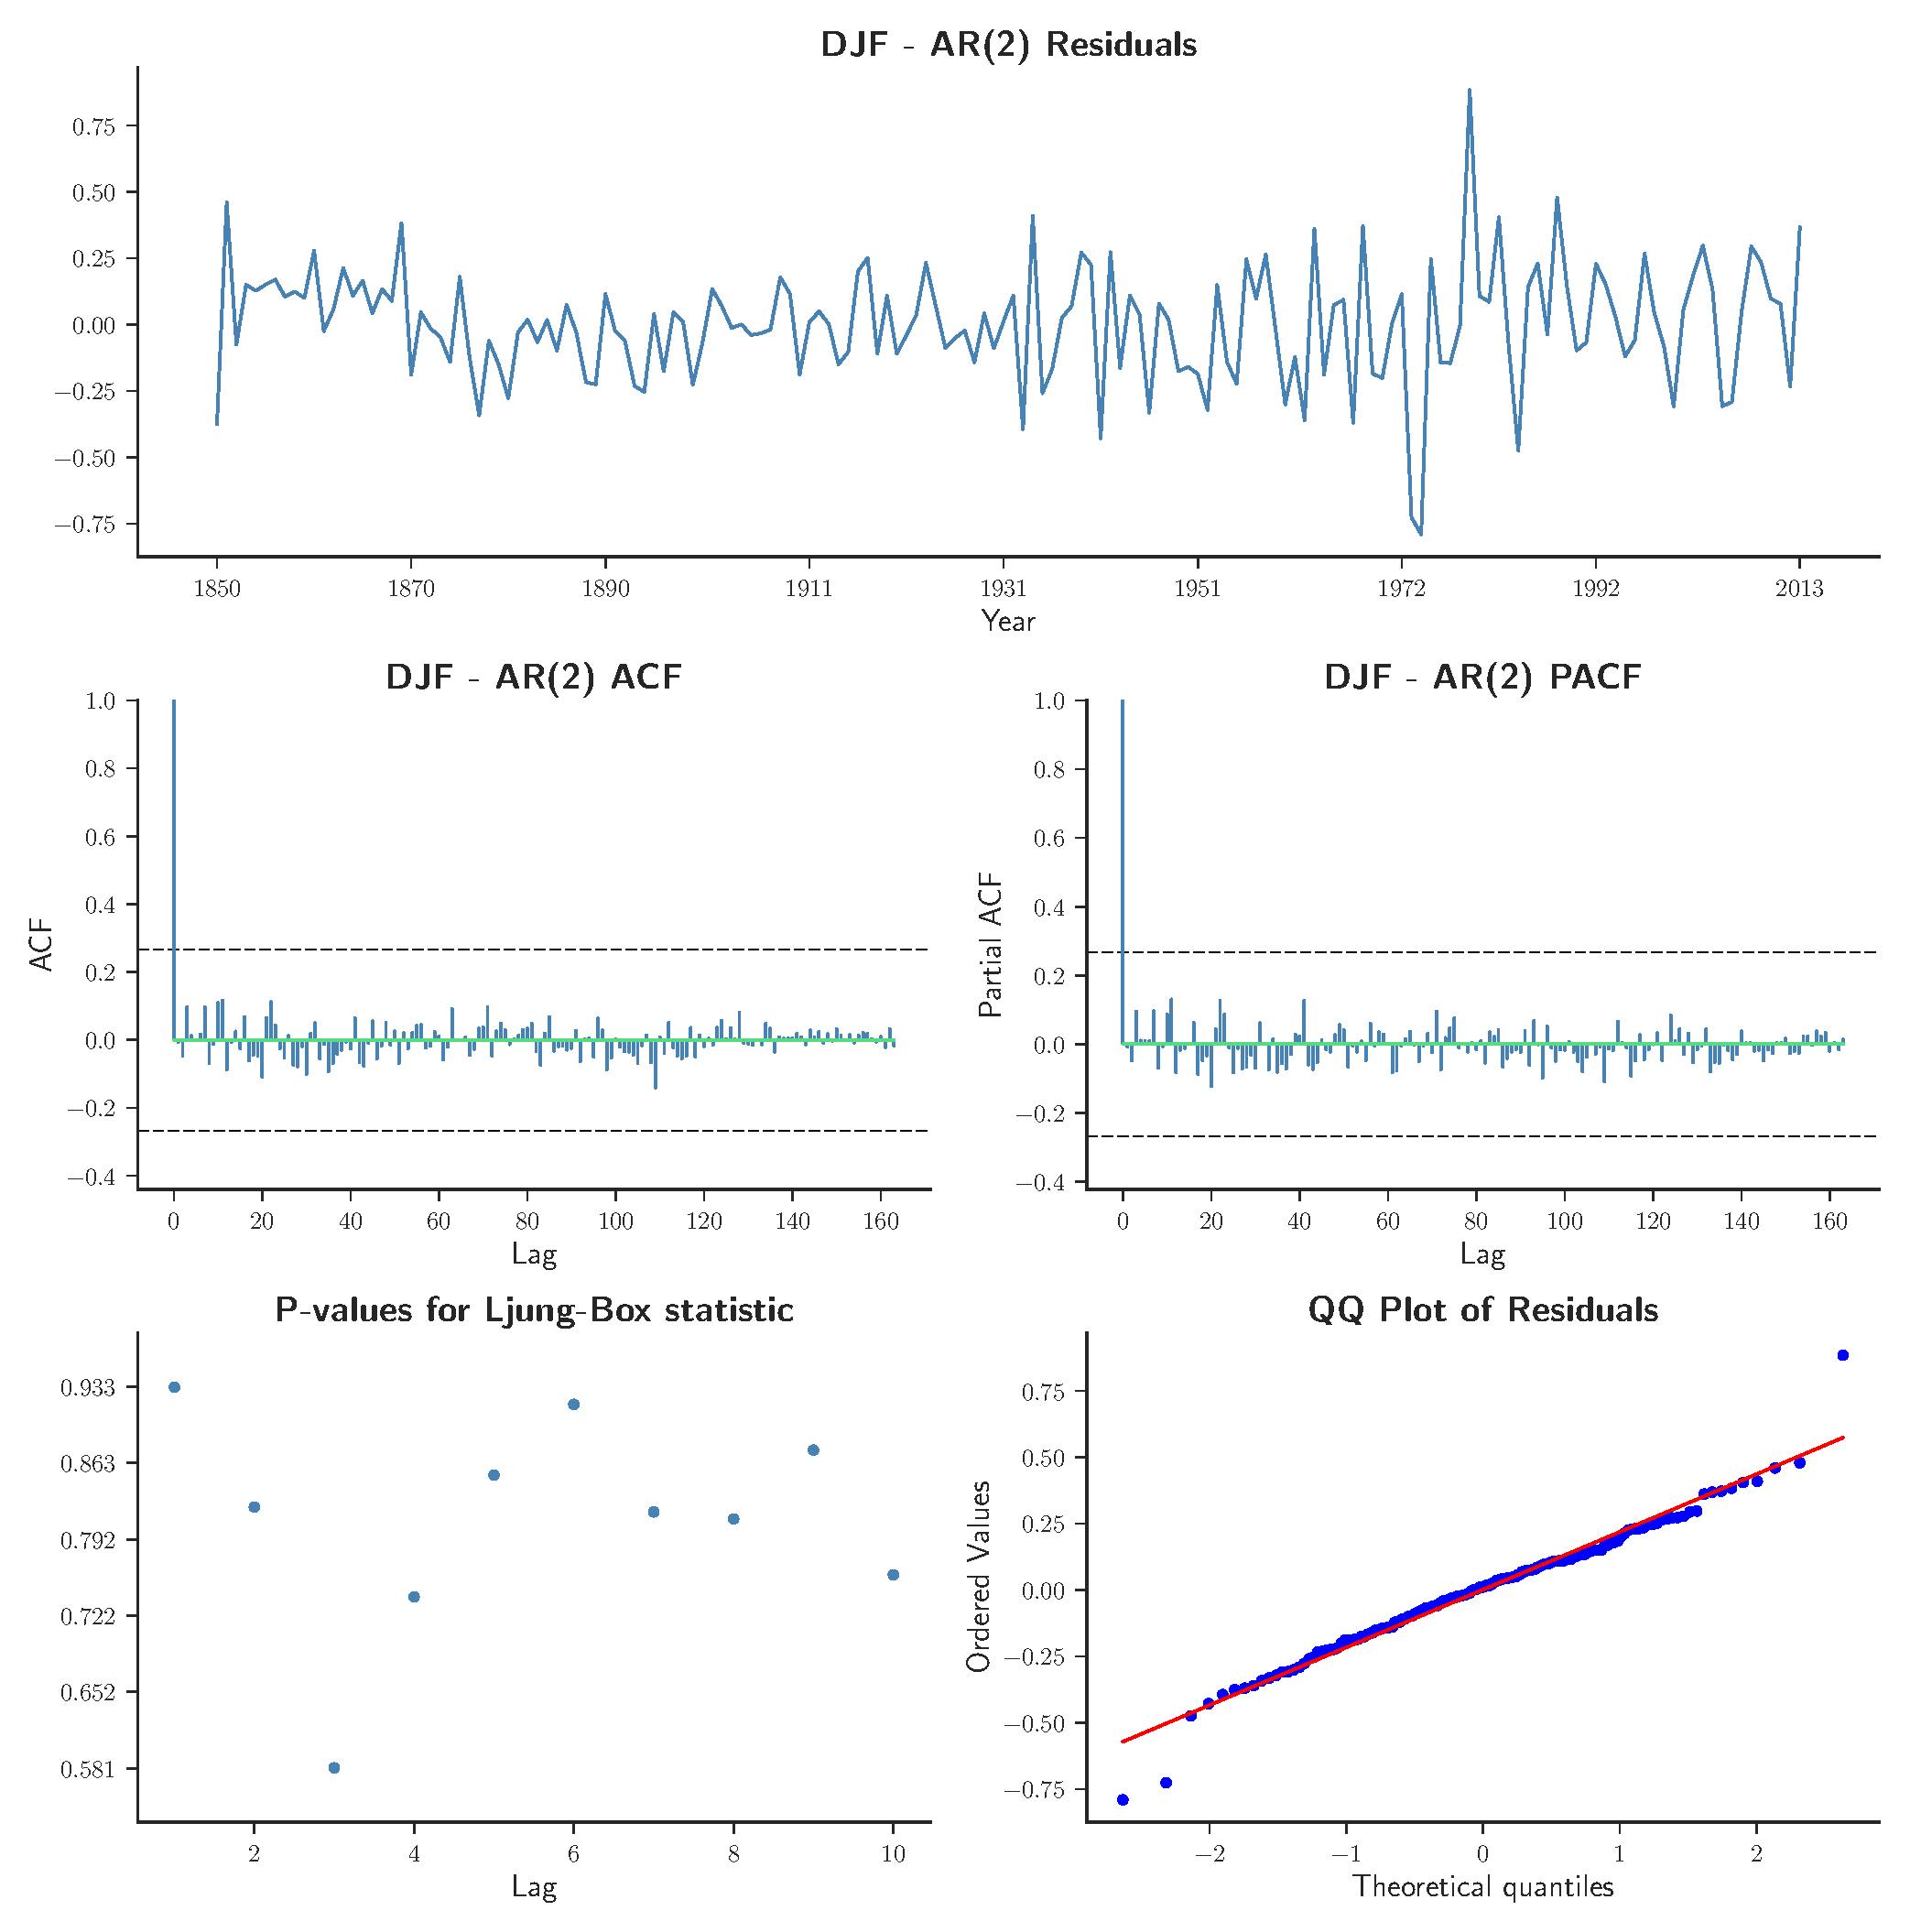
\includegraphics[width=1\textwidth,center]{figs/djf_res}
  \caption{JJA - ACF and PACF}\label{djf_res}
\end{figure}

\begin{figure}[!htbp]
  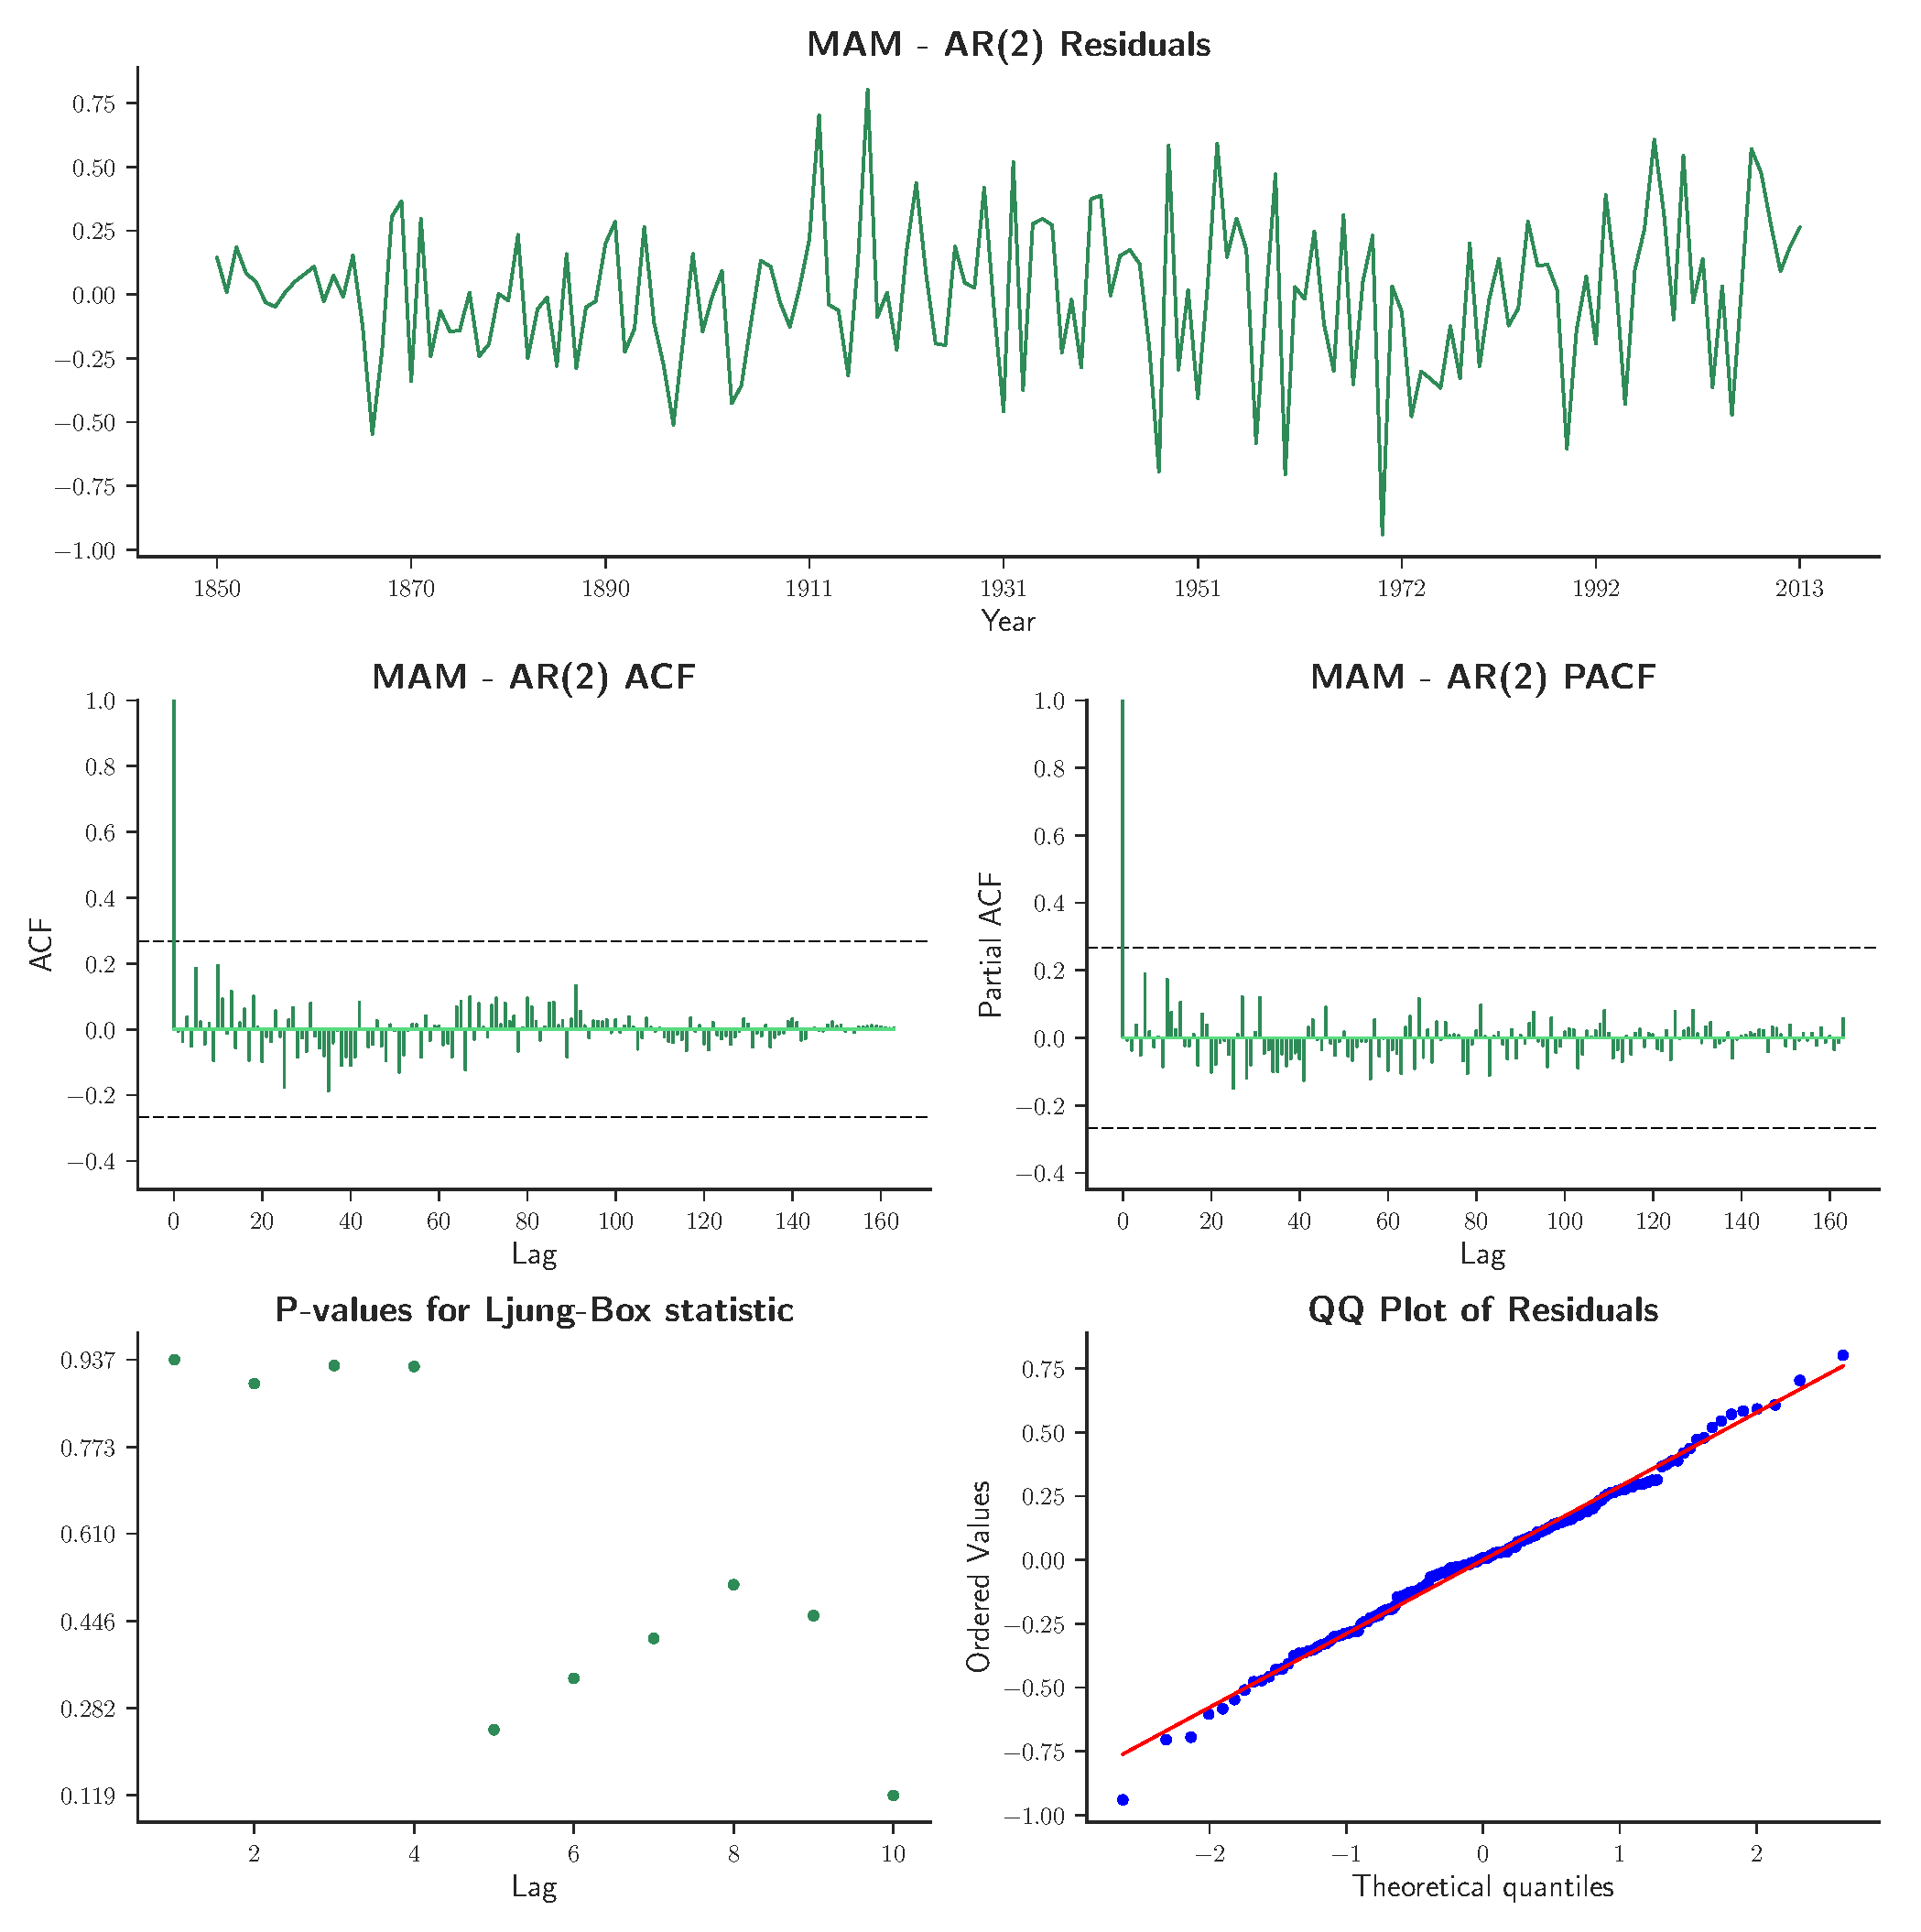
\includegraphics[width=1\textwidth,center]{figs/mam_res}
  \caption{JJA - ACF and PACF}\label{mam_res}
\end{figure}

\begin{figure}[!htbp]
  \centering
  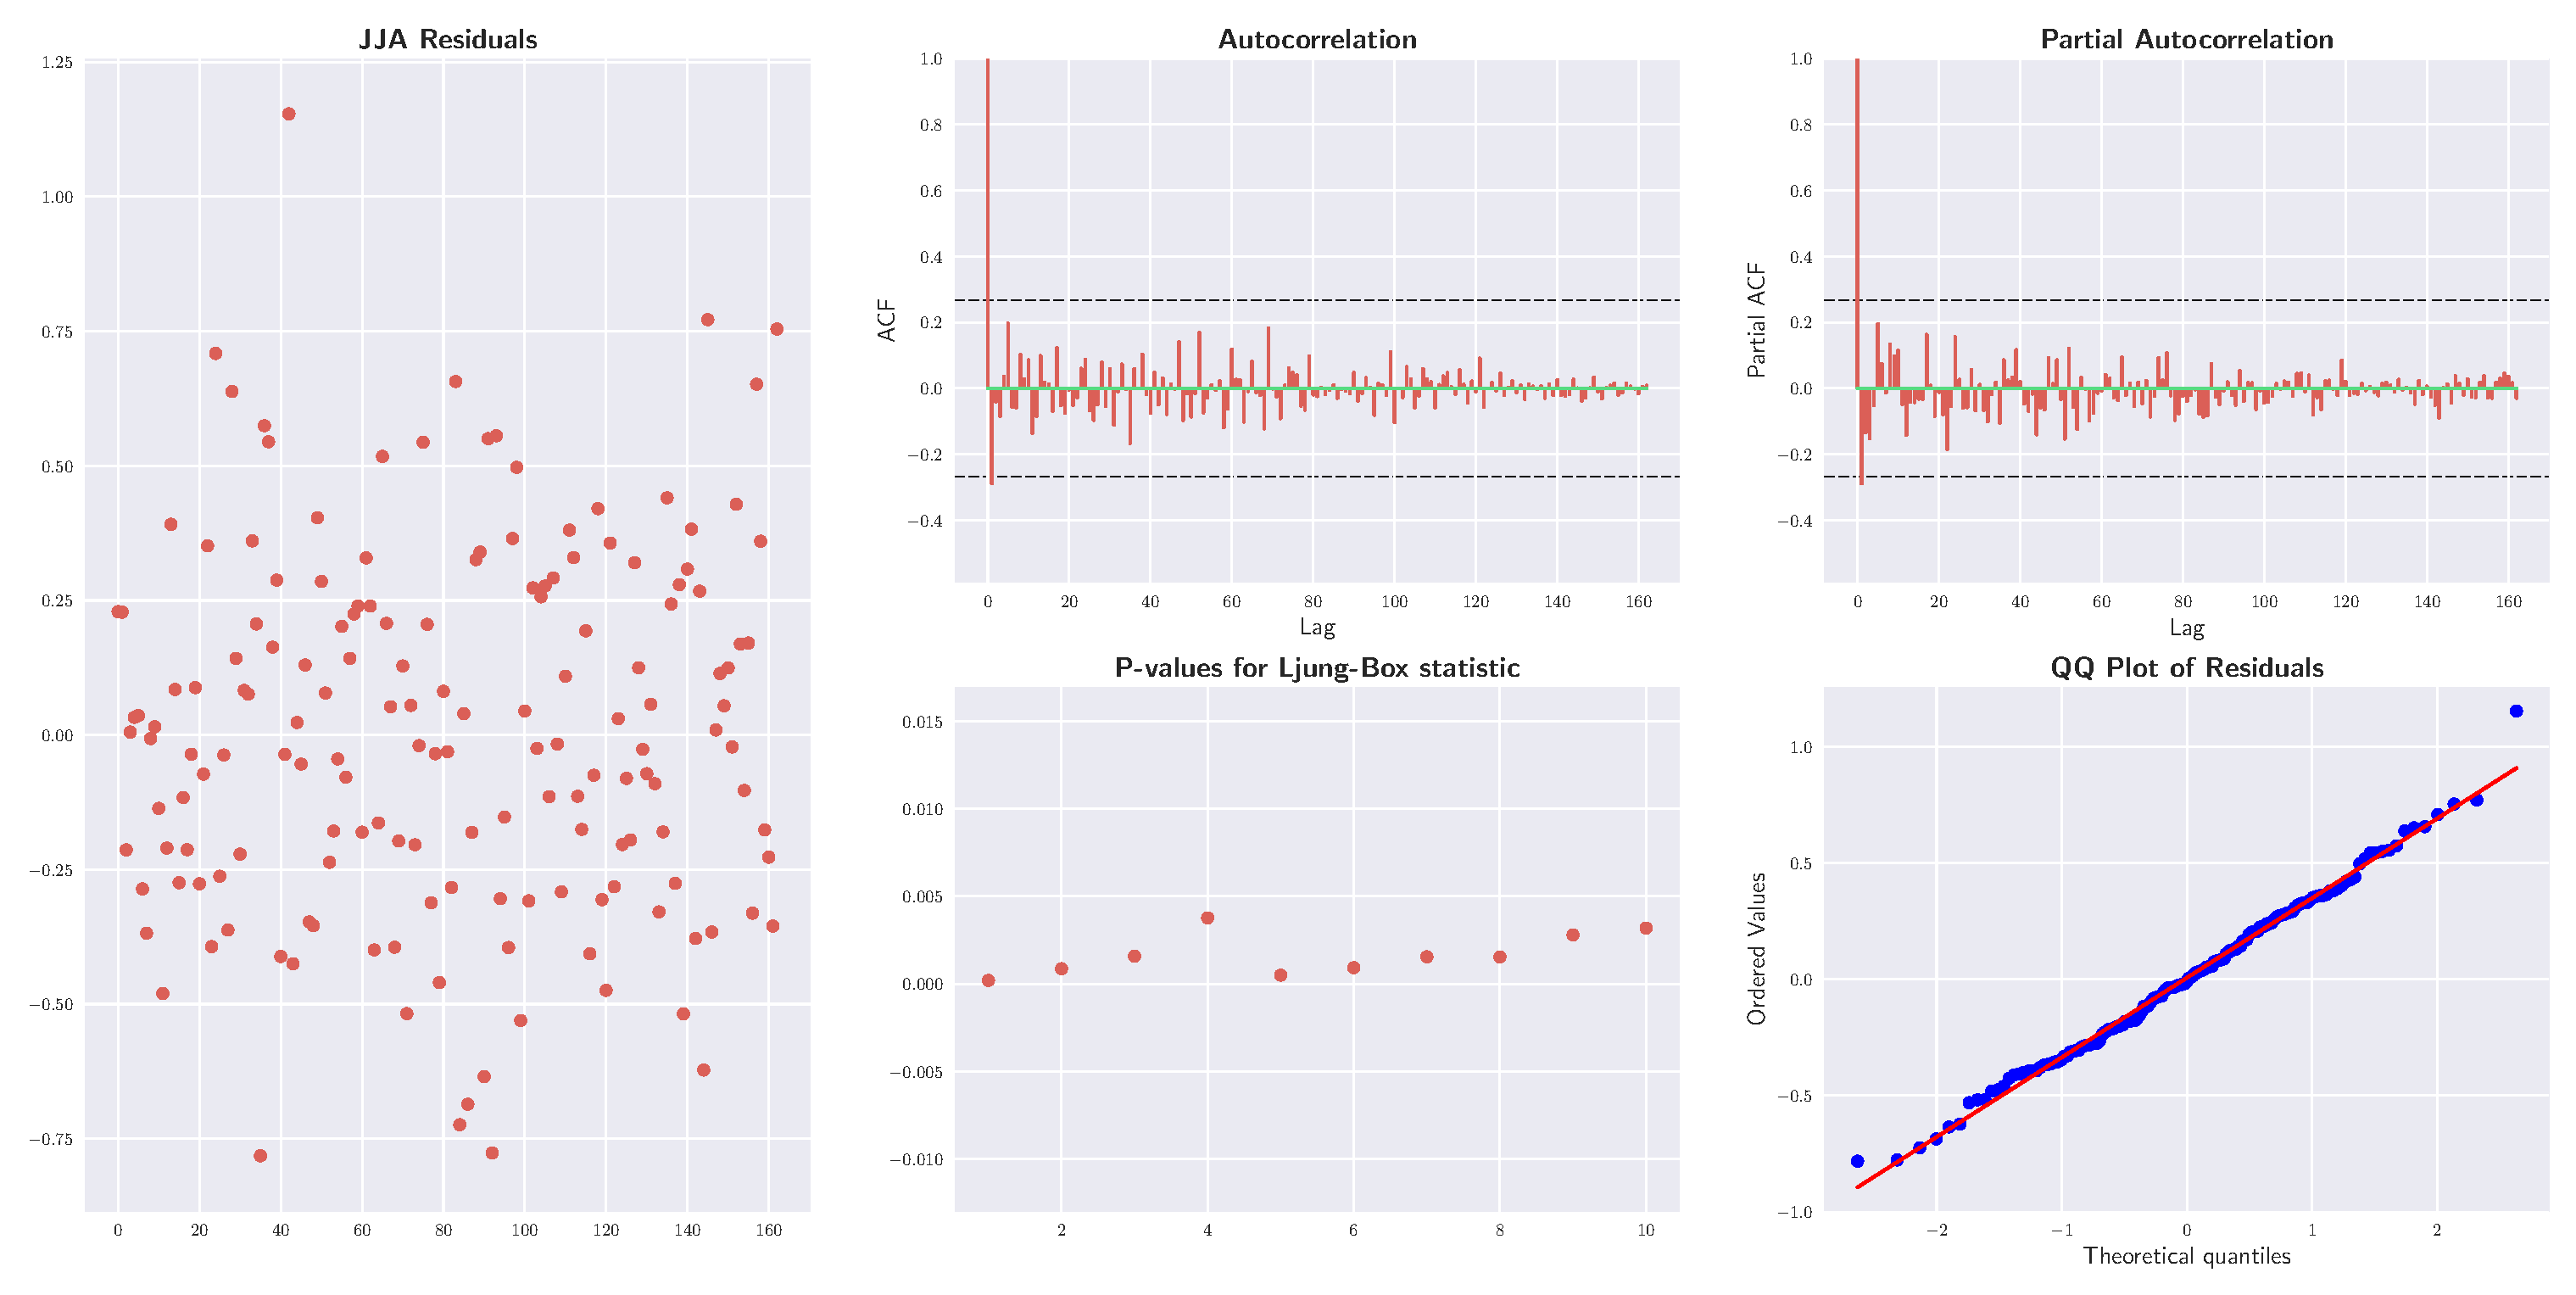
\includegraphics[width=1\textwidth,center]{figs/jja_res}
  \caption{JJA - ACF and PACF}\label{jja_res}
\end{figure}

\begin{figure}[!htbp]
  \centering
  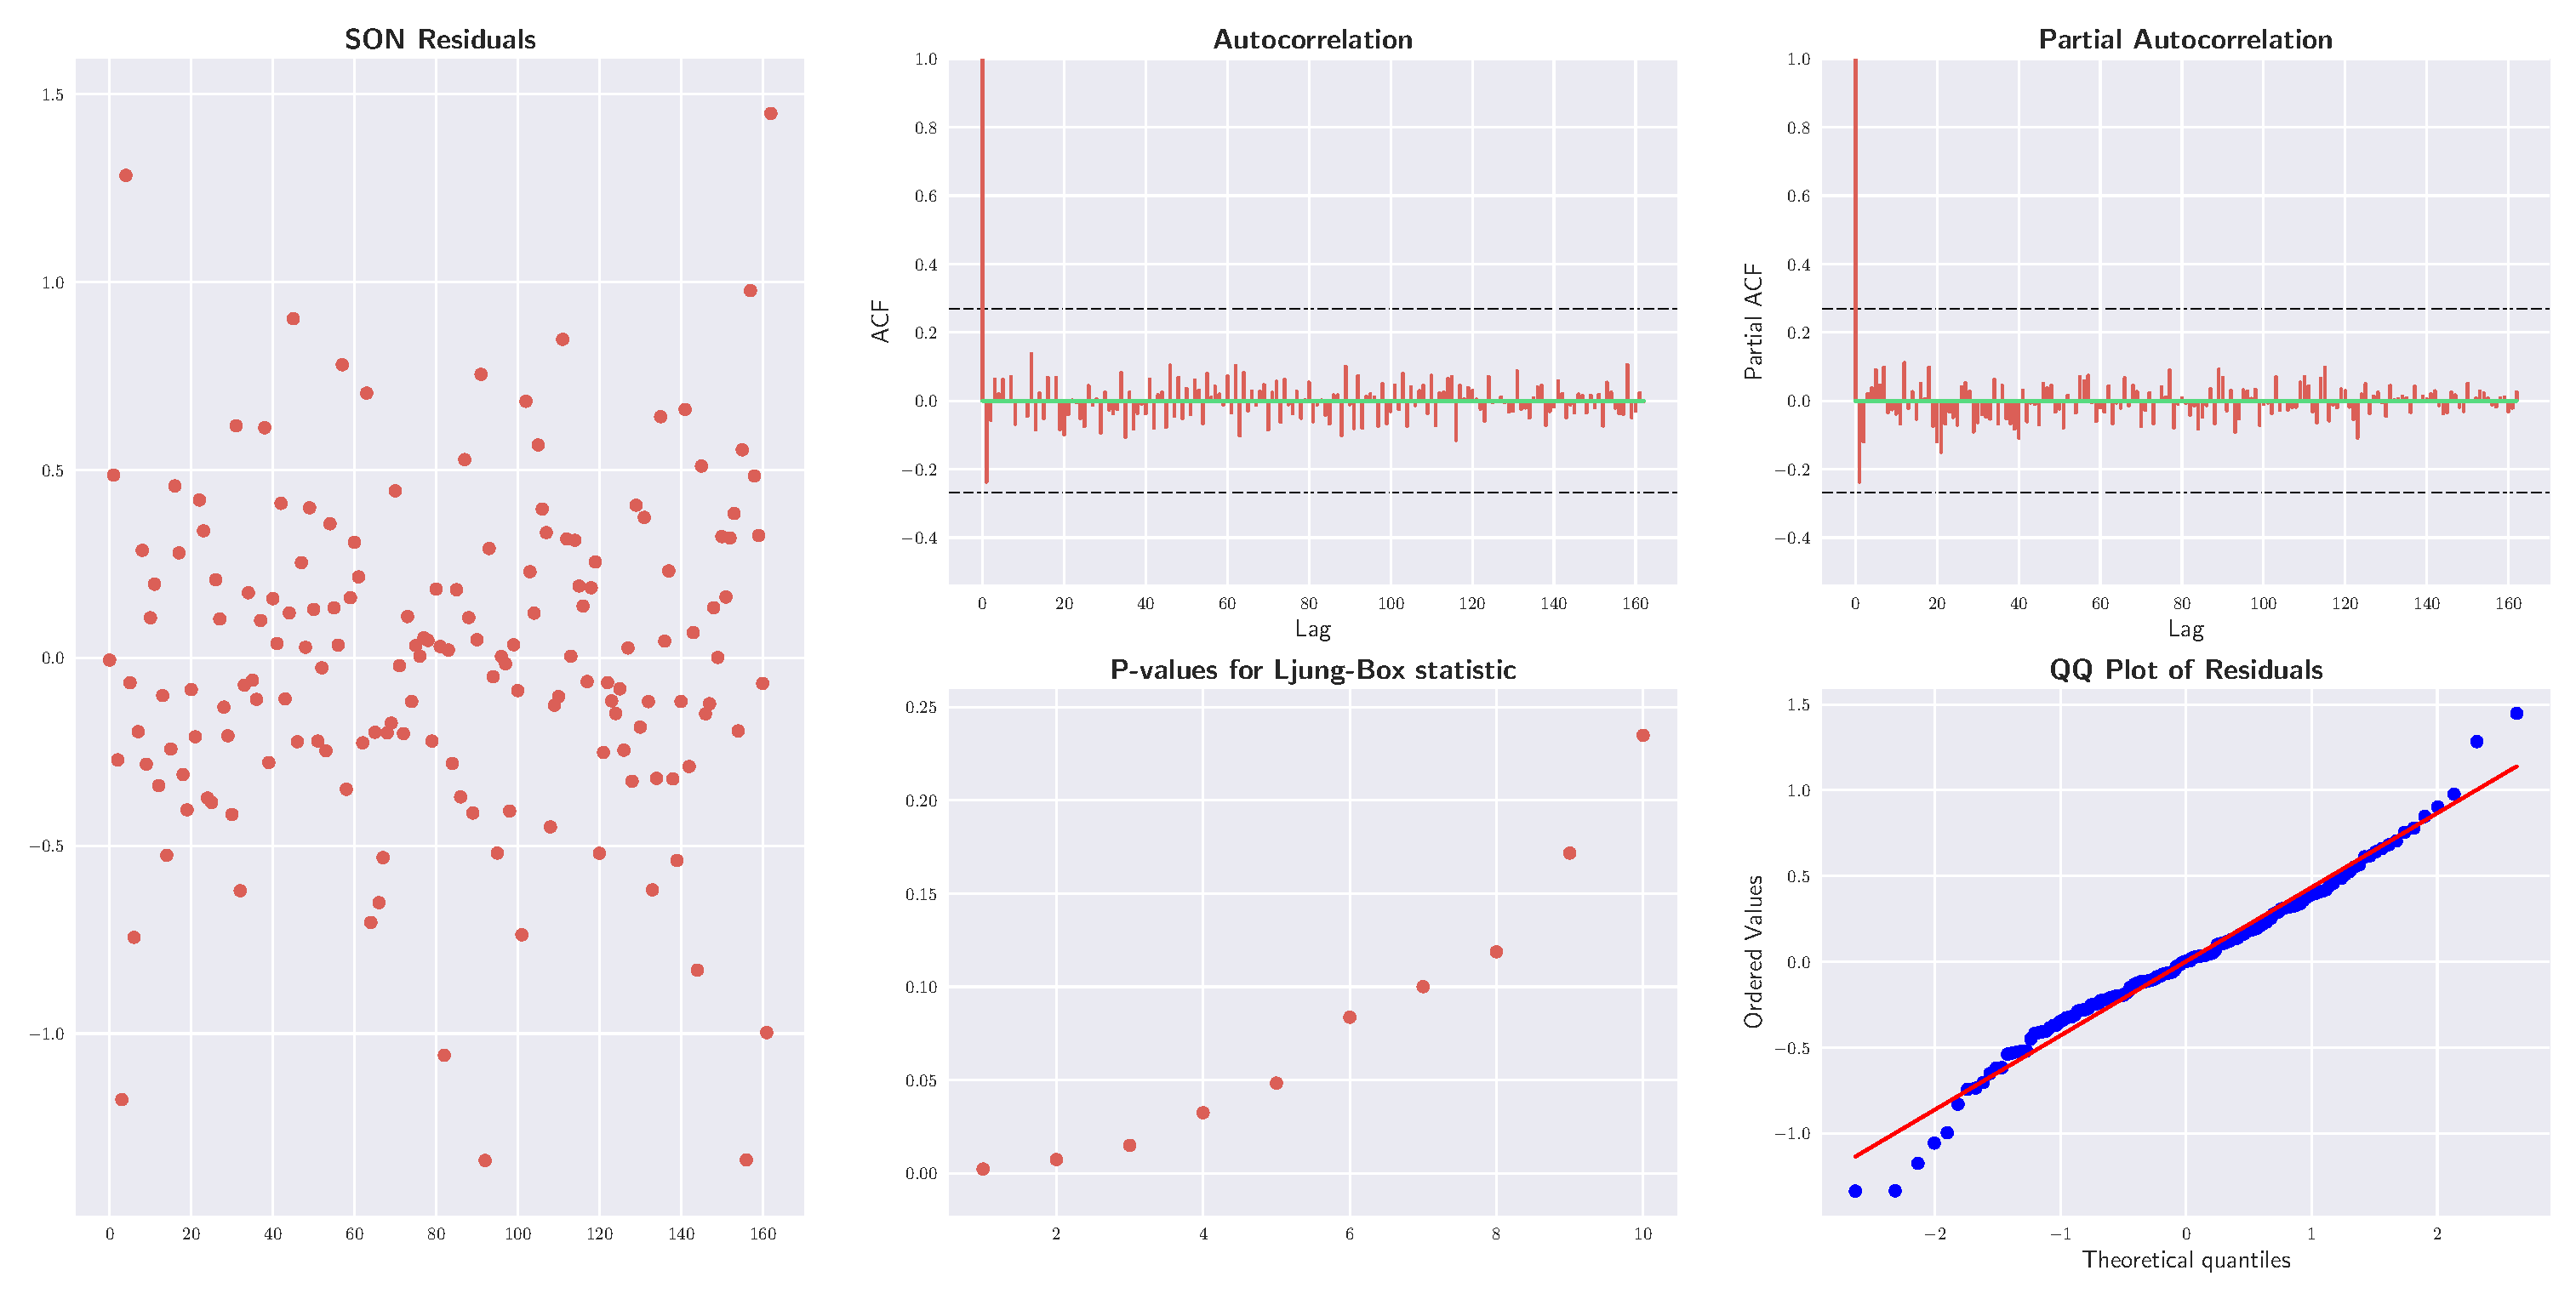
\includegraphics[width=1\textwidth,center]{figs/son_res}
  \caption{JJA - ACF and PACF}\label{son_res}
\end{figure}

The Ljung-Box test for JJA and SON suggest that there is not enough evidence that the residuals of our AR(2) models esemble white noise, hence they exhibit serial correlation. However for DJF and MAM, there is significant evidence that our AR(2) models resemble white noise after certain lags.

The residuals for DJF suggest white noise for lags 1 through 10. For MAM, there is an oscilitaing pattern of whiteness for each lag.

The results of our models capture the majority of the structure for DJF and MAM. However, the residuals for JJA and SON suggest a more complex mean or dependence structure.

\section{Conclusion}
In summary, we have demonstrated the use of non-parametric change point detection to detect interesting climate phenomenons that lead to significant changes in climate trend. Linear spline regression was used to capture the linear trend in the Arctic sea ice concentration. This resulted in detrending our series to investigate the periodicity. We have found that the retreat of the Arctic sea ice has a dominant frequency of 1 every 42 years for JJA.

\bibliographystyle{apalike}
\bibliography{arctic_refs}

\end{document}